\section{Biased\-Node\-Selector Class Reference}
\label{class_biased_node_selector}\index{BiasedNodeSelector@{BiasedNodeSelector}}
A node selector that does a specified number of rounds ignoring terminals.  


{\tt \#include $<$Node\-Selector.h$>$}

Inheritance diagram for Biased\-Node\-Selector::\begin{figure}[H]
\begin{center}
\leavevmode
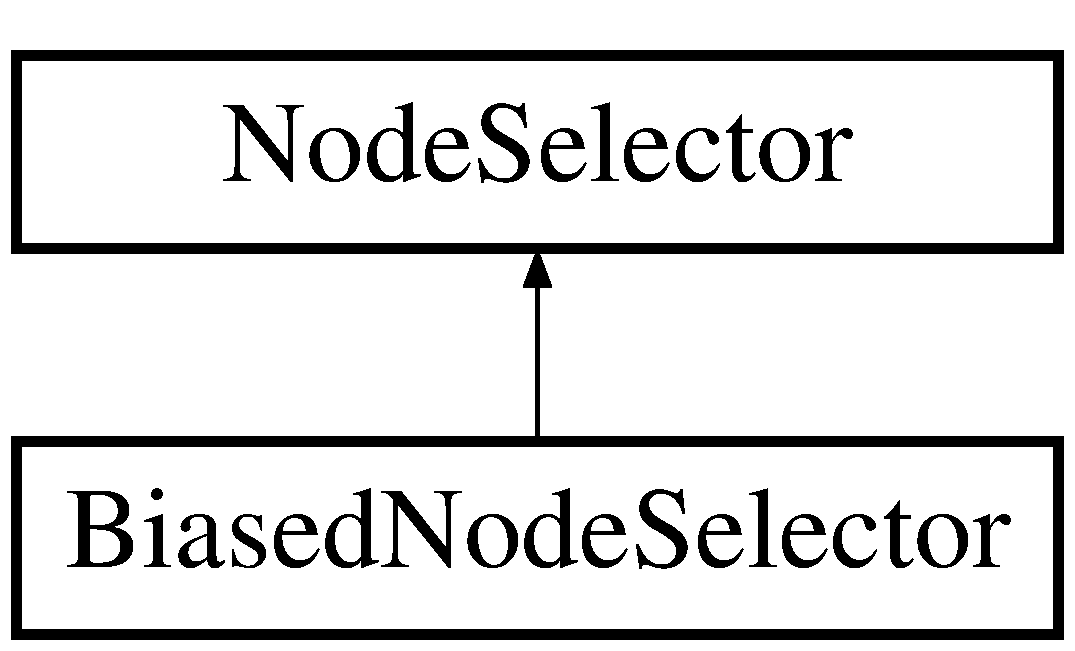
\includegraphics[height=2cm]{class_biased_node_selector}
\end{center}
\end{figure}
\subsection*{Public Member Functions}
\begin{CompactItemize}
\item 
{\bf Biased\-Node\-Selector} (unsigned n)\label{class_biased_node_selector_a1}

\item 
Node\-Selection {\bf select\_\-node} (Sym sym) const \label{class_biased_node_selector_a2}

\end{CompactItemize}
\subsection*{Public Attributes}
\begin{CompactItemize}
\item 
unsigned {\bf n\-Rounds}\label{class_biased_node_selector_o0}

\end{CompactItemize}


\subsection{Detailed Description}
A node selector that does a specified number of rounds ignoring terminals. 



Definition at line 55 of file Node\-Selector.h.

The documentation for this class was generated from the following files:\begin{CompactItemize}
\item 
Node\-Selector.h\item 
Node\-Selector.cpp\end{CompactItemize}
